\section{Experiments}

\subsection{Data}

We're using the \textit{BigEarthNet dataset} \cite{bigearthnet} for our evaluations. The goal is to use the model as a feature generator and use these features for solving the multi-label classification problem with 19 classes and also 43 classes from BigEarthNet. This dataset contains around 550,000 image patches from Sentinel-I and Sentinel-II with multi-class labels for every image. We are going to use the \textit{Sentinel-I} images for our experiments.

The data is split into train and test set based on the implementation from the \href{https://torchgeo.readthedocs.io/en/latest/api/datasets.html#bigearthnet}{torchgeo repository}. The train dataset contains around 270,000 and the test dataset has 125,000 images.

There are high differences in the occurrence of certain classes in the dataset (see Fig. \ref{fig:class-distribution}). There are, for example, only a few images with wetlands, beaches, and moors. The metrics during the evaluation have to account for this.

\begin{figure}[h]
  \centering
  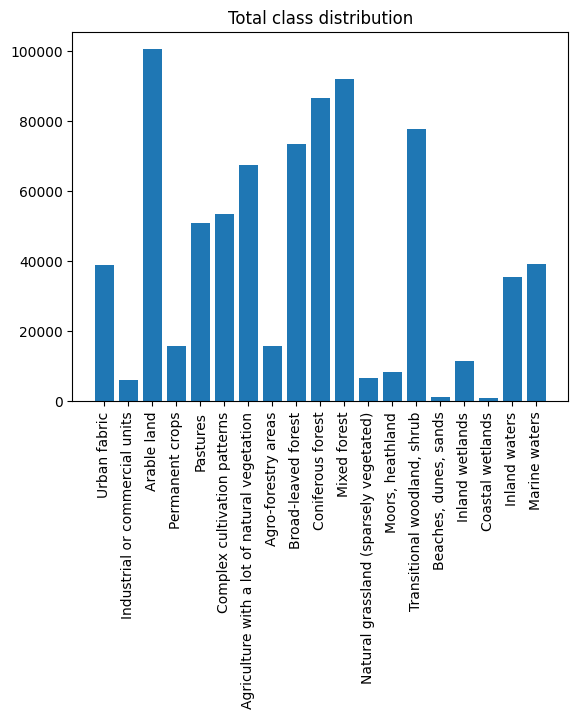
\includegraphics[width=0.8\columnwidth]{images/class_distribution.png}
  \caption{Distribution of the classes in the train dataset. This is a multiclass dataset so one can have multiple classes.}
  \label{fig:class-distribution}
\end{figure}

\begin{figure}[h]
  \centering
  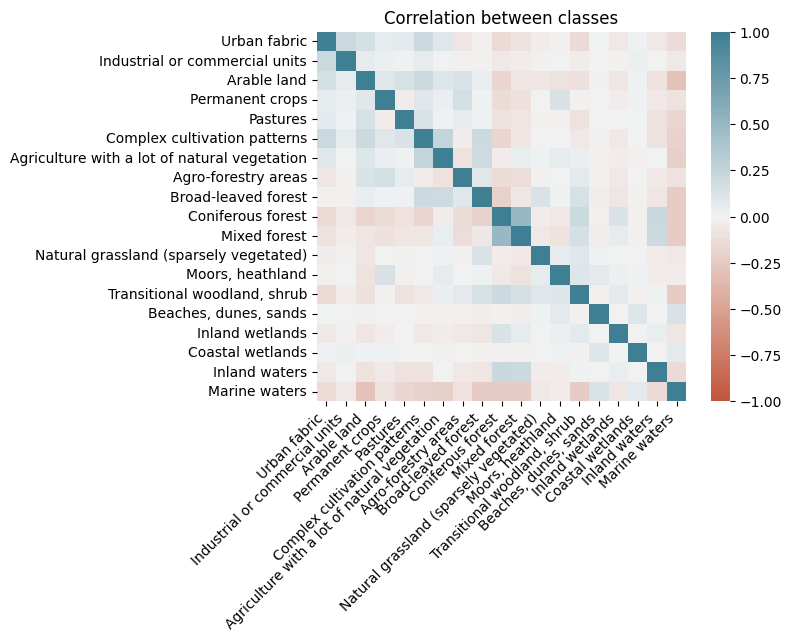
\includegraphics[width=\columnwidth]{images/correlation.png}
  \caption{Correlation of classes in the train dataset}
  \label{fig:correlation}
\end{figure}

We analyzed the correlation between classes of BigEarthNet and the results are displayed in Fig. \ref{fig:correlation}. The classes are mostly uncorrelated with some exceptions like the high likelihood that coniferous forests are usually also mixed forests and marine waters are mostly not in the same images as all the other vegetation forms.

\subsection{Performance Metrics}

We decided to compute multiple metrics for evaluating the performance of the models in the classification tasks. We provide results for \textit{f2-micro, f2-macro} (\href{https://scikit-learn.org/stable/modules/generated/sklearn.metrics.fbeta_score.html}{Implementation}), \textit{hamming-loss}, and \textit{precision} scores (\href{https://scikit-learn.org/stable/modules/generated/sklearn.metrics.precision_score.html}{Implementation}). We also calculate precision and f1 scores for individual classes.

\subsection{Results}

First, we calculated feature vectors using DOFA for all the images in BigEarthNet (Sentinel-I) and saved them for further use. All the following analyses use these vectors for visualizations or the downstream classification task.

\subsubsection{UMAP Feature analysis}

\begin{figure*}[h]
  \centering
  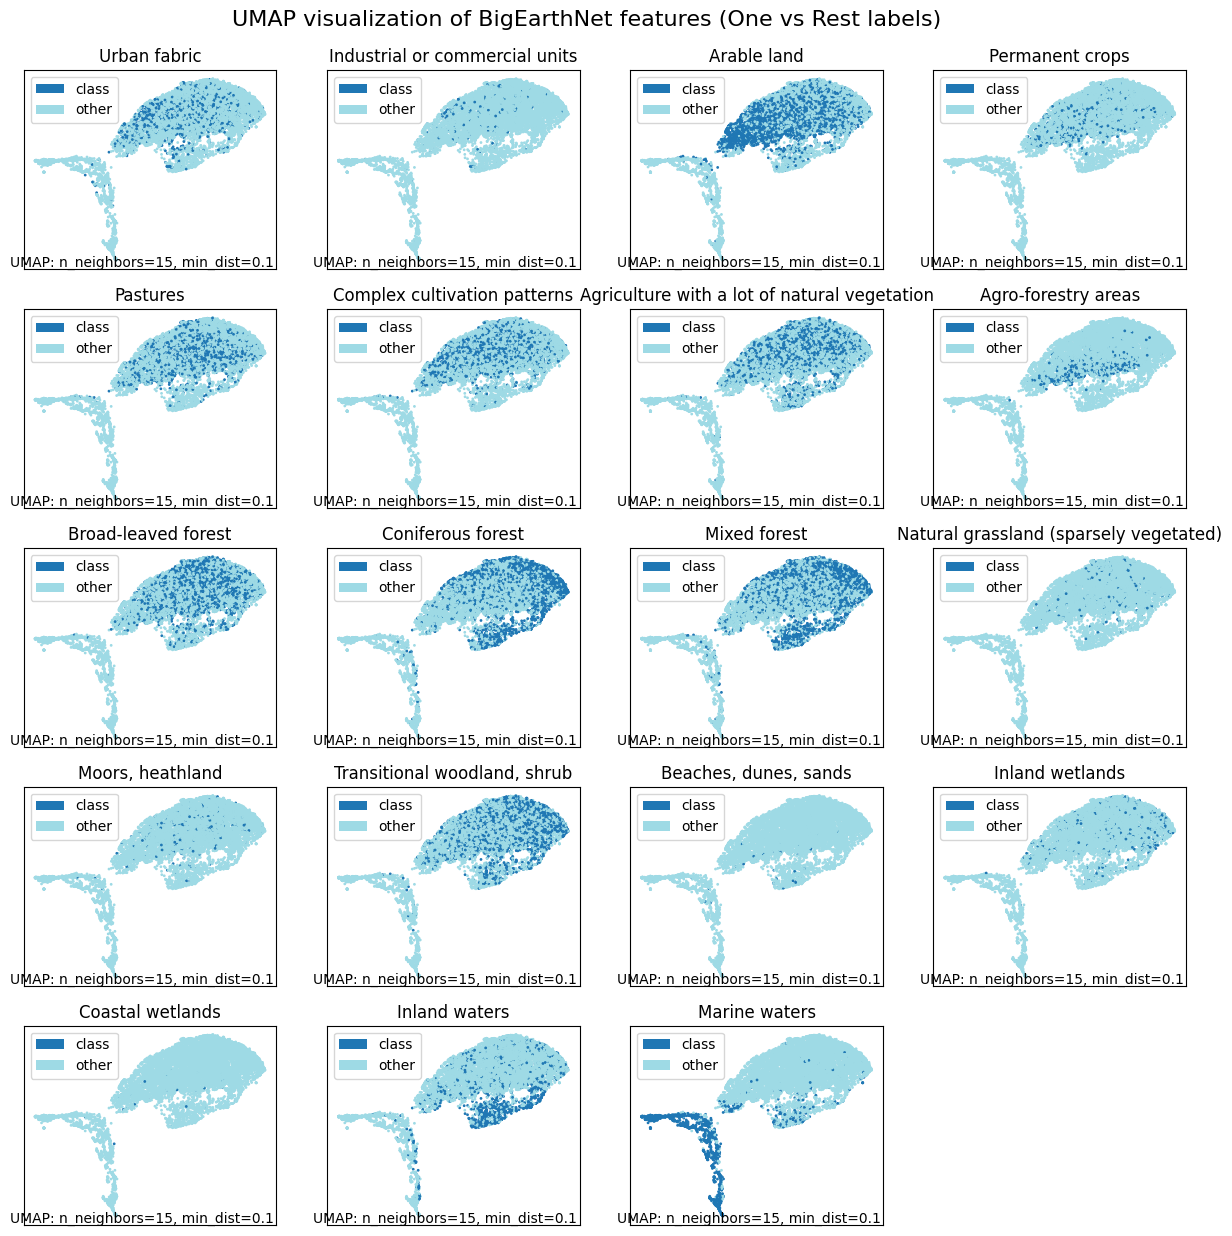
\includegraphics[width=0.8\textwidth]{images/umap.png}
  \caption{Visualization of the 19 classes in a UMAP transformed space (one vs. rest)}
  \label{fig:umap}
\end{figure*}

In Fig. \ref{fig:umap} are the occurrences of different classes in a UMAP transformed 2D space visualized. Because one image has multiple labels, we chose the visualization via multiple charts. In this visualization, we expect different classes to be located in different data cloud regions. As we can see, this assumption holds for a lot of the classes. Most notably, we have a separate region for all marine water images (right bottom chart). As we've seen in Fig. \ref{fig:correlation}, this class is negatively correlated with most of the other classes, so a separation in this visualization is plausible. It appears that arable land is more on the left side of the largest region, while forests, woodlands, etc. are more on the right side.

With the results of this visualization, we expect that the feature vectors of DOFA capture the semantic meaning of the different images, and it should be possible to train a classifier on top of them.

\subsubsection{Classification}

We used the feature vectors of DOFA to train different ML algorithms for the given classification task. All the approaches use the same data split. In Table \ref{fig:test-results} are the final results of these experiments.

\begin{table*}[h]
  \centering
  \begin{tabular}{lcccccc}
    \textbf{} & \textbf{$F^2_{macro}$ (\%)} & \textbf{$F^2_{micro}$ (\%)} & \textbf{hamming loss} & \textbf{$P_{macro}$ (\%)} & \textbf{$P_{micro}$ (\%)} \\
    \hline
    Random Forest & 21.4 & 35.8 & 0.123 & 52 & \textbf{72} \\
    Linear Probing & 22.9 & 35.3 & 0.124 & 49 & 70 \\
    MLP & \textbf{34.5} & \textbf{47.8} & \textbf{0.113} & \textbf{58} & 71 \\
  \end{tabular}
  \caption{Test results of different classification approaches on the 19-class multi-label classification task. Some classes contain so few examples that they are not in the test dataset and receive an $F^2$ score of 0.}
  \label{fig:test-results}
\end{table*}

There are notable differences in the performance of the chosen approaches. MLP has the best performance over most of the metrics. However, the random forest classifier and linear probing also have similar scores in $P_{micro}$ and $P_{macro}$. All classifiers have significant differences between their micro and macro averaged $F^2$ scores. When we compare the $F^2$ scores per class, we can see the cause for these values (Fig. \ref{fig:scores-by-class}): There is a high variance in the performance across classes, which ranges from 0\% $F^2$ score to about 90\% $F^2$ score. This leads to the different averaging variants resulting in different scores. We can also see that MLP manages to achieve higher scores than the linear classifier over more classes. Additionally, the low performing classes are mostly similar and correlate to the classes with low-data availability. It seems that the labels were not enough to learn all of the classes well.

\begin{figure}[h]
  \centering
  \begin{minipage}[b]{0.48\columnwidth}
    \centering
    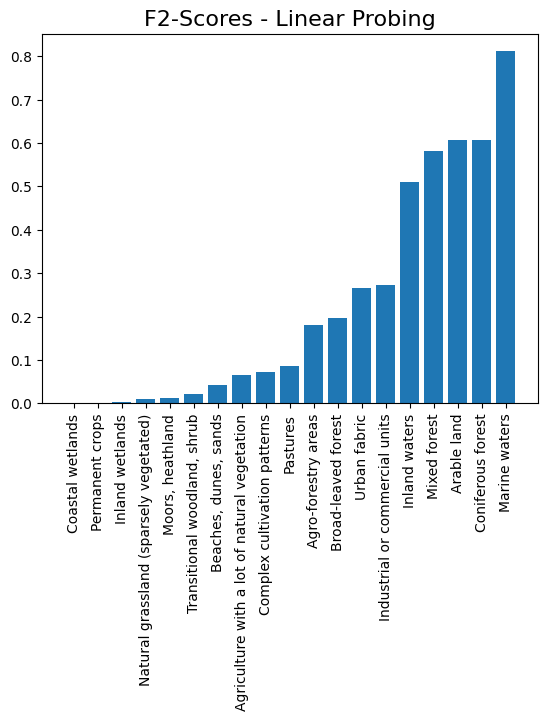
\includegraphics[width=\columnwidth]{images/Linear Probing - f2 scores.png}
  \end{minipage}
  \begin{minipage}[b]{0.48\columnwidth}
    \centering
    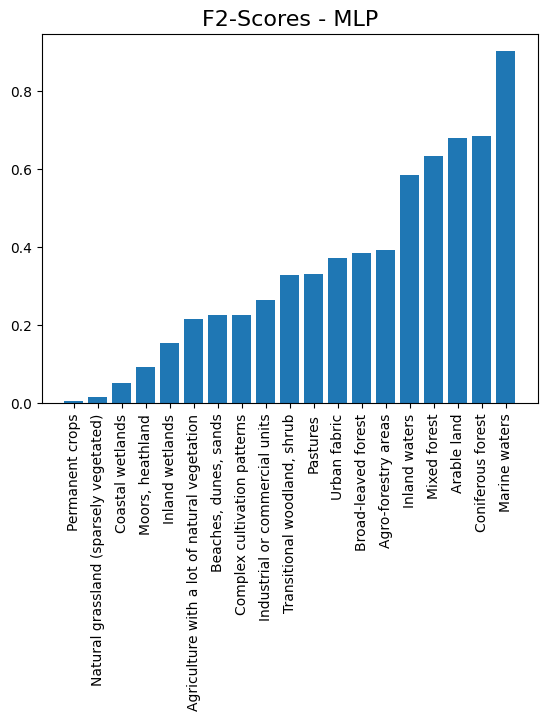
\includegraphics[width=\columnwidth]{images/MLP - f2 scores.png}
  \end{minipage}
  \caption{$F^2$ scores for every class (19 in total). Left side for the linear classifier, right side for the MLP classifier.}
  \label{fig:scores-by-class}
\end{figure}

We can conclude that the features generated by the DOFA model are not well linearly separable across all classes and only some achieve an $F^2$ score of over 50\%. The MLP model can separate more complex data and therefore reaches a better performance.

Random forest classifiers can separate high dimensional data, but in this case, as seen in Table \ref{fig:test-results}, their scores are on the same level as the linear classifier. % WHY????

\begin{table*}[h]
  \centering
  \begin{tabular}{lcccccc}
    \textbf{} & \textbf{$F^2_{macro}$ (\%)} & \textbf{$F^2_{micro}$ (\%)} & \textbf{hamming loss} & \textbf{$P_{macro}$ (\%)} & \textbf{$P_{micro}$ (\%)} \\
    \hline
    Random Forest & 9.46 & 33.73 & 0.056 & 24 & \textbf{71} \\
    Linear Probing & 12.63 & 36.54 & 0.057 & 28 & 66 \\
    MLP & 15.45 & 44.46 & 0.052 & \textbf{38} & \textbf{71} \\
    \hline
    COMP \cite{bigearthnet-comparison-model} & \textbf{52.8} & \textbf{62.3} & \textbf{0.04} & / & / \\
  \end{tabular}
  \caption{Test results of different classification approaches on the 43-class multi-label classification task. For comparison, we provide the results of a specialized model for this task \cite{bigearthnet-comparison-model}. This comparison is only meant as a reference as this paper uses the Sentinel-II images of BigEarthNet, which includes more spectral bands.}
  \label{fig:test-results-43}
\end{table*}

In Table \ref{fig:test-results-43} we provide test results for the multi-label classification task with 43 classes of BigEarthNet \cite{bigearthnet}. The results are expected worse than on the 19-class variant, as this is a more complex task. We can see that the DOFA model isn't able to keep up with a specialized model, e.g. \cite{bigearthnet-comparison-model} even though this comparison has its limitations as this paper used the Sentinel-II images.

\begin{figure}[h]
  \centering
  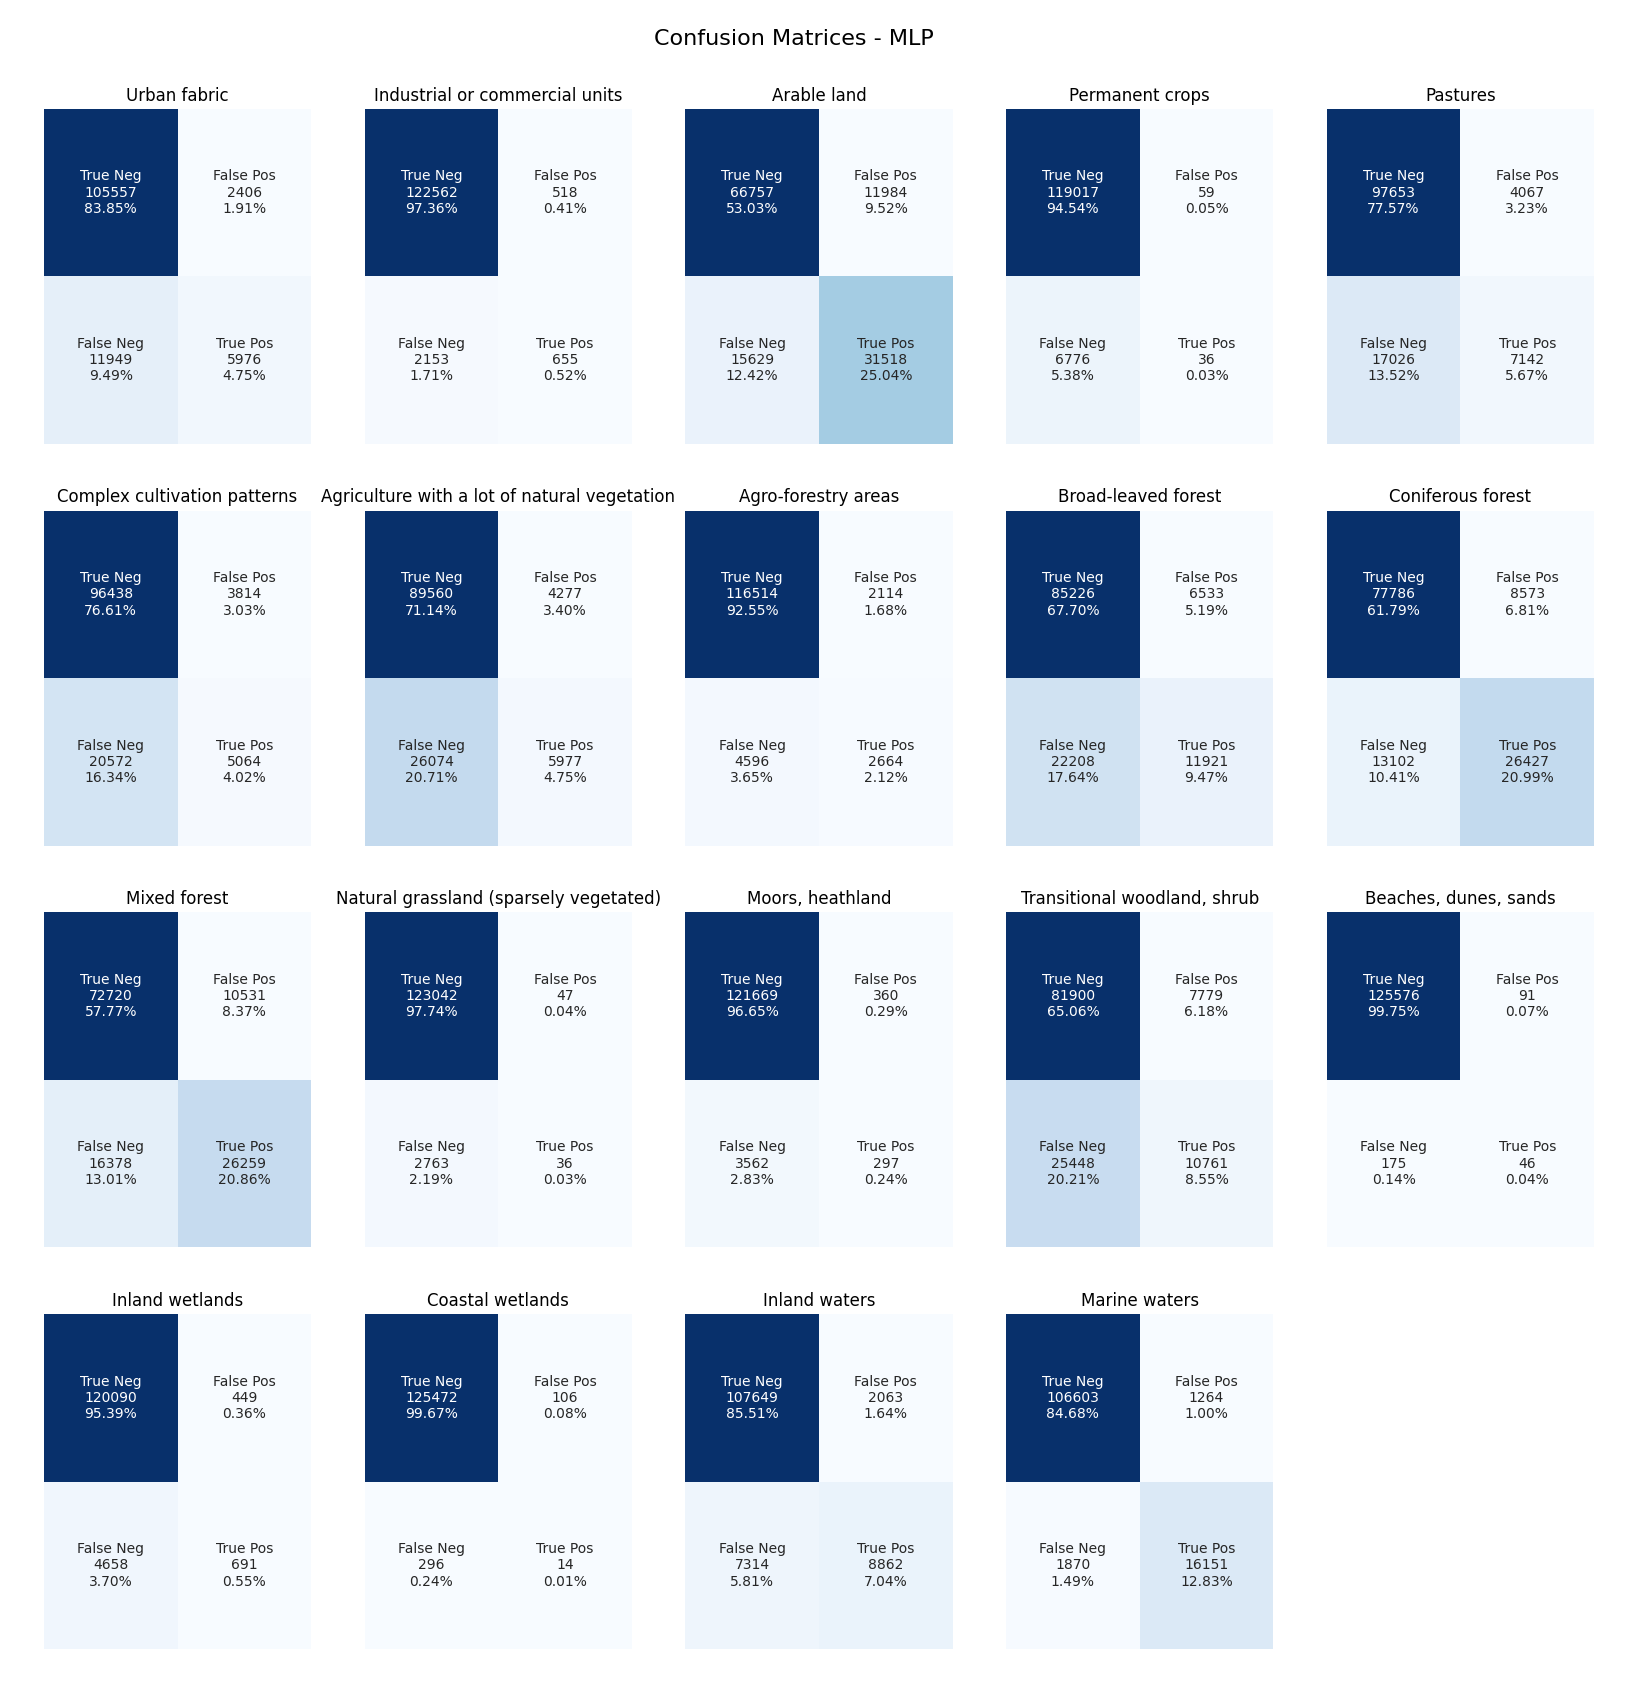
\includegraphics[width=\columnwidth]{images/MLP - confusion matrix.png}
  \caption{Confusion matrices of the MLP classifier on the test set with 19 classes. The matrices are calculated separately for each class.}
  \label{fig:confusion-matrix}
\end{figure}

In Fig. \ref{fig:confusion-matrix}, we see the confusion matrices of the best model over the 19 classes. With 19 classes, it is sensible that most of the classes are quite uncommon, which results in a lot of true negatives. It is interesting to see that most of the errors come from false negatives, which means that the model is unable to detect certain classes in an image.